\documentclass[a4paper,11pt]{article}
% ---- graphiques
\usepackage[pdftex]{graphicx}
\usepackage{wrapfig}
\usepackage{color}

% for latex2html
\usepackage{html}

% for accents
\usepackage[latin1]{inputenc}
\usepackage[T1]{fontenc}

\definecolor{darkgreen}{rgb}{0,0.4,0}
\definecolor{darkblue}{rgb}{0,0,0.4}
\definecolor{darkgray}{rgb}{0.2,0.2,0.2}

% ---- inclusion de codes
\usepackage{listings}
\lstset{showstringspaces=false,tabsize=4,basicstyle=\scriptsize\sffamily,breaklines=true,breakatwhitespace=true,framexleftmargin=5mm, frame=shadowbox, framesep=1pt,rulesepcolor=\color{darkgray},rulesep=.5pt,keywordstyle=\bf\color{blue},commentstyle=\color{magenta},stringstyle=\color{red},numbers=left,numberstyle=\tiny,numbersep=5pt,columns=flexible}

\lstdefinestyle{bash}{language=bash}
\lstdefinestyle{Perl}{language=Perl}
\lstdefinestyle{C++}{language=C++,emph={__global__,__shared__,__syncthreads,blockIdx,threadIdx,float3,float4},emphstyle=\bf\color{darkgreen}}
\lstdefinestyle{DTD}{language=XML}
\lstdefinestyle{XML}{language=XML,usekeywordsintag=false,markfirstintag=true}
%begin{latexonly}
\newcommand{\includecode}[2]{
\lstinputlisting[style=#1]{#2}
}
%end{latexonly}
\begin{htmlonly}
\newcommand{\includecode}[2]{  \htmladdnormallink{#2}{../../#2} }
\end{htmlonly}
%\lstnewenvironment{code}{}{}
\lstnewenvironment{code_bash}{\lstset{style=bash}}{}
\lstnewenvironment{code_perl}{\lstset{style=Perl}}{}
\lstnewenvironment{code_cpp}{\lstset{style=C++}}{}
\lstnewenvironment{code_dtd}{\lstset{style=DTD}}{}
\lstnewenvironment{code_xml}{\lstset{style=XML}}{}

\newcommand{\textcode}[1]{{\sf #1}}




\newcommand{\sofa}{SOFA}
\newcommand{\todo}[1]{}
\newcommand{\eg}{\textit{e.g.} }


% macros mathematiques
\newcommand{\ma}[1]{\ensuremath{\mathbf {#1}}}
\newcommand{\ve}[1]{\ensuremath{\mathbf {#1}}}

\usepackage{amsmath}
\usepackage{amsfonts}
\usepackage{amssymb}

% character styles
\newcommand{\bm}[1]{\ensuremath{\mathbf{{#1}}}}
\newcommand{\mcal}[1]{\mbox{$\mathcal #1$}} % rondes math
\newcommand{\bmcal}[1]{\mbox{\boldmath $\mathcal #1$}} % rondes grasses math
\newcommand{\ensemble}[1]{\mbox{$\mathbb{#1}$}}
\newcommand{\RRR}{\mbox{$\ensemble{R}^3$}} 


% d�finitions
\newcommand{\definition}[2]{\index{#1}{\bf #1}: #2}
\newcommand{\voc}[1]{\index{#1}#1}
\newcommand{\bvoc}[1]{\index{#1}{\bf #1}}

% misc
\newcommand{\EV}[1]{\stackrel{\rightarrow}{#1}}  % espace vectoriel
\newcommand{\EA}[1]{#1}                          % espace affine

% vectors, matrices
%\newcommand{\point}[1]{\mbox{$#1$}}          % un point
\newcommand{\point}[1]{\ensuremath{#1}}          % un point
\newcommand{\mat}[1]{\bm{#1}}         % matrice
\newcommand{\matnm}[3]{\bm{#1_{#2\times #3}}}  % matrice n lignes , m colonnes
\newcommand{\vect}[1]{\bm{#1}}        % vecteur 
%\newcommand{\vecf}[1]{\stackrel{\rightarrow}{#1}}  % vecteur avec fleche
\newcommand{\vecf}[1]{\mbox{$\overrightarrow{#1}$}}  % vecteur avec fleche
\newcommand{\ident}[1]{\bm{I_{#1}}}   % identit� en dimension n
\newcommand{\inv}[1]{#1^{-1}}         % matrice inverse
\newcommand{\psinv}[1]{#1^{+}}        % matrice pseudo-inverse
\newcommand{\transp}[1]{#1^T}         % transpos�e de 1
\newcommand{\trace}[1]{tr(#1)}        % trace
\newcommand{\deter}[1]{\mbox{$|#1|$}}       % determinant
\newcommand{\oppvec}[1]{\mbox{$\left( \vect {#1} \wedge \right)$}}  % operateur matriciel de produit vectoriel

% bases, reperes
\newcommand{\vecin}[2]{\mbox{${}^{#2}#1$}}    % vecteur 1 dans repere 2
\newcommand{\Base}[1]{\ensuremath{\mathcal B_{#1}}} % Symbole du repere 1
\newcommand{\chbase}[3]{\mbox{${}_{#2}^{#3}\mat{#1}$}}  % operateur 1 fait le passage de la base 3 vers la base 2
%\newcommand{\pchbase}[2]{\chbase{\mat{B}}{#1}{#2}}  % matrice de passage de la base 2 vers la base 1
\newcommand{\pchbase}[2]{\chbase{B}{#1}{#2}}  % matrice de passage de la base 2 vers la base 1
\newcommand{\Rep}[1]{\ensuremath{\mathcal R_{#1}}} % Symbole du repere 1
\newcommand{\rep}[1]{\Rep{#1}}                 % Symbole du repere 1
%\newcommand{\pchrep}[2]{\chbase{\mat{F}}{#1}{#2}}  % matrice de passage du repere 1 vers le repere 2, F comme Frame
\newcommand{\pchrep}[2]{\chbase{\bm{C}}{#1}{#2}}  % matrice de passage du repere 2 vers le repere 1

%% Operateur de passage du repere 1 par rapport a 2
%\newcommand{\ChgRep}[2]{\mbox{\boldmath $R_{#1}^{#2}$}}

% rotations	
%\newcommand{\rot}[2]{\mbox{$\mat{R}_{#1,#2}$}}      % rotation vectorielle
\newcommand{\rot}[2]{\ensuremath{\mat{R}_{#1,#2}}}      % rotation vectorielle
\newcommand{\rota}[3]{\mbox{$\mat{R}_{#1,#2,#3}$}}  % rotation affine

% translation
\newcommand{\trans}[2]{\mbox{$\chbase{\vect{t}}{#1}{#2}$}} % passage de #1 vers #2 par une translation, ou translation du repere #2 par rapport au repere #1

% vitesses et acc�l�rations
\newcommand{\VRep}[2]{\mbox{\boldmath $\dot R_{#1}^{#2}$}} % vitesse du repere 1 par rapport a 2 
%\newcommand{\Point}[2]{\mbox{\boldmath ${#1}^{#2}$}}  % Coordonnees d'un point 1 dans un repere 2
\newcommand{\Point}[2]{\mbox{$\vecin{\bm{#1}}{#2}$}}  % Coordonnees d'un point 1 dans un repere 2
\newcommand{\VPoint}[2]{\mbox{\boldmath ${\dot #1}_{/#2}$}} % Vitesse d'un point par rapport � un repere
\newcommand{\APoint}[2]{\mbox{\boldmath ${\ddot #1}_{/#2}$}} % Acceleration d'un point par rapport � un repere

% cinematique du solide
\newcommand{\derivedans}[2]{\mbox{$\dot{#1}^{(#2)}$}}  % derivee du vecteur 1 dans repere 2
\newcommand{\fixedans}[2]{\mbox{$#1_{\in #2}$}}        % vecteur 1 fixe dans repere 2
\newcommand{\vecom}{\mbox{$\bm{\Omega}$}}  % omega de 1 par rapport a 2
\newcommand{\vecrot}[2]{\mbox{$\vecom_{#1/#2}$}}  % omega de 1 par rapport a 2
\newcommand{\accrot}[2]{\mbox{$\dot{\vecom}_{#1/#2}$}}  % omega de 1 par rapport a 2
\newcommand{\vfdans}[3]{\mbox{$\vec V^{#2/#3}_{#1}$}}    % vitesse de 1 fixe dans 2 par rapport a 3
\newcommand{\afdans}[3]{\mbox{$\vec \Gamma^{#2/#3}_{#1}$}}    % acceleration de 1 fixe dans 2 par rapport a 3
\newcommand{\vmdans}[2]{\mbox{$\vec V^{/{#2}}_{#1}$}}    % vitesse de 1 mobile dans 2
\newcommand{\amdans}[2]{\mbox{$\vec \Gamma^{/#2}_{#1}$}}    % acceleration de 1 mobile dans 2

% chaines articulees
\newcommand{\liaison}[2]{\mbox{$\mathcal L_{#1,#2}$}}  % liaison du pere 1 vers fils 2 (et repere intermediaire)
\newcommand{\liaisonprime}[2]{\mbox{$\mathcal L'_{#1,#2}$}}  % deuxieme repere intermediaire de la liaison du pere 1 vers fils 2
\newcommand{\liaisonP}[2]{\mbox{$\mathcal L_{#1,#2}$}}  % Repere dans pere 1 de la liaison vers fils 2 
\newcommand{\liaisonC}[2]{\mbox{$\mathcal L'_{#1,#2}$}}  % Repere dans fils de la liaison du pere 1 vers fils 2 
%\newcommand{\transP}[2]{\pchrep{\liaisonP{#1}{#2}}{#1}}  % Matrice du repere dans pere de la liaison du pere 1 vers fils 2 
%\newcommand{\transC}[2]{\pchrep{\liaisonC{#1}{#2}}{#2}}  % Matrice du repere dans pere de la liaison du pere 1 vers fils 2 
%\newcommand{\transPC}[2]{\pchrep{\liaisonC{#1}{#2}}{\liaisonP{#1}{#2}}}  % matrice de passage entre repere liaison dans fils et repere de liaison dans pere
\newcommand{\transP}[2]{\chbase{C_p}{#2}{#1}}  % Matrice du repere dans pere de la liaison du pere 1 vers fils 2 
\newcommand{\transC}[2]{\chbase{C_c}{#2}{#1}}  % Matrice du repere dans pere de la liaison du pere 1 vers fils 2 
\newcommand{\transPC}[2]{\chbase{C_l}{#2}{#1}}  % matrice de passage entre repere liaison dans fils et repere de liaison dans pere
% \pchrep{fils}{pere} = \liaisonP{pere}{fils}\deplPC{pere}{fils}\liaisonC{pere}{fils}


\newcommand{\pctab  }{\hspace{0.15in}      }  % Pseudo-code indentation.
\newcommand{\code}[1]{ 
\begin{makeimage}
\begin{tabbing} \pctab \= \pctab \= \pctab \= \pctab \= \pctab \= \pctab \= \pctab \kill
#1
\end{tabbing}
\end{makeimage}
}
 % This file is in parent directory. Your TEXINPUTS environment variable must include .. to reach this file. Example: setenv TEXINPUTS ..:../..:${TEXINPUTS}

% ---- format de page A4
	\setlength{\textwidth }{16cm}	% largeur de ligne
	\setlength{\textheight}{23cm}   % hauteur du texte
	\setlength{\oddsidemargin}{0cm} % marge pages impaires
	\setlength{\evensidemargin}{0cm}% marge pages paires
	\setlength{\topmargin}{0cm} 	
	\setlength{\headheight}{14pt} 
	\setlength{\headsep}{0.5cm} 

\newenvironment{componentoption}[1]%
{\textbf{#1}\newline}
{\newline}

\newcommand{\aliases}[1] {\newline \textit{Aliases - } #1}
\newcommand{\defaultvalue}[1] {\newline \textit{Default Value - } #1}
\newcommand{\valuetype}[1] {\newline \textit{Value Type - } \textbf{#1}}

\usepackage{caption}
\usepackage{subcaption}
\usepackage{hyperref}

\begin{document}
\raggedright

\title{Flexible}
\author{SOFA}

\maketitle

\begin{abstract}

\end{abstract}

\newcommand{\flexible}{\em{Flexible}}

\newcommand{\pos}{\vect{x}}
\newcommand{\dx}{\vect{\Delta x}}
\newcommand{\xcur}{\vect{x}_{n}}
\newcommand{\xnext}{\vect{x}_{n+1}}
\newcommand{\vel}{\vect{v}}
\newcommand{\dv}{\vect{\Delta v}}
\newcommand{\vcur}{\vect{v}_{n}}
\newcommand{\vnext}{\vect v_{n+1}}
\newcommand{\acc}{\vect{a}}
\newcommand{\force}{\vect{f}}
\newcommand{\forcext}{\vect{f}_{ext}}
\newcommand{\lam}{\vect{\lambda}}
\newcommand{\lcur}{\lam_{n}}
\newcommand{\lnext}{\lam_{n+1}}
\newcommand{\avlam}{\bar{\lam}}
\newcommand{\fcur}{\vect{f}_{n}}
\newcommand{\fnext}{\vect f_{n+1}}
\newcommand{\Minv}{\mat M^{-1}}
\renewcommand{\P}{\mat P}
\newcommand{\cmp}{c}
\newcommand{\dampingratio}{d}

\newcommand{\p}{\vect{p}}  % moving point
\newcommand{\polynomial}[2]{{#1}^{#2}}  % polynomial coordinates of a point
\newcommand{\pp}{\polynomial{\p}{*}}  % polynomial coordinates of point p
\newcommand{\ppinit}{\polynomial{\pinit}{*}}  % polynomial coordinates of point \bar p
\newcommand{\initial}[1]{\bar{#1}}  % initial coordinates of a point
\newcommand{\pinit}{\initial{\p}}  % initial coordinates of a point
\newcommand{\pref}{\initial{\p}}  % reference (undeformed) point
\newcommand{\disp}{\vect{u}}  % displacement
\newcommand{\f}{\vect{f}}    % forces

\newcommand{\dof}{q}           % independent DOF
\newcommand{\dofinit}{\initial\dof}           % independent DOF
\newcommand{\dofpos}{\ensuremath{\vect{x}} }           % posititon in 3d of an independent DOF
\newcommand{\dofposinit}{\initial\dofpos }           % posititon in 3d of an independent DOF
\newcommand{\pdofposinit}{\polynomial{\dofposinit}{*}}
\newcommand{\pdofposinitcov}[1]{\polynomial{\dofposinit_#1}{*}\polynomial{\dofposinit_#1}{*T}}
\newcommand{\vdof}{\vect{\dof}}           % vector of independent DOF
\newcommand{\vdofinit}{\vect{\dofinit}}          % independent DOF
\newcommand{\fdof}{\f}           % force on independent DOF
\newcommand{\vfdof}{\vect{\fdof}}           % vector of independent DOF force
\newcommand{\dofm}{\mat{A}}         % DOF matrix
\newcommand{\dofmrel}{\mat{A^r}}         % DOF matrix
\newcommand{\mparam}{\theta}           % material parameter
\newcommand{\vmparam}{\vect{\mparam}}           % material points
\newcommand{\defograd}{F}           % deformation gradient
\newcommand{\fdefograd}{\mathcal{F}}           % deformation gradient generalized force
\newcommand{\strain}{\epsilon}           % strain
\newcommand{\stress}{\sigma}           % stress
\newcommand{\W}{\mathcal{W}}           % elastic energy
\newcommand{\C}{\mat{C}}           % damping matrix

\newcommand{\volume}{\ensuremath{\mathcal{V}}} 
\newcommand{\sample}{\ensuremath{{\mathcal{V}e}}} 
\newcommand{\vol}{\ensuremath{\Delta v}}
\newcommand{\volmass}{\ensuremath{\rho}}
\newcommand{\mass}{\mat{M}}

\newcommand{\ddof}{\ensuremath{\dot{\dof}}}
\newcommand{\dddof}{\ensuremath{\ddot{\dof}}}
\newcommand{\diff}{\ensuremath{\boldsymbol{\nabla}_i}}

\newcommand{\Jt}{\J^T}

\newcommand{\mCoord}{\vect{\Theta}}
\newcommand{\shapef}{w}

\newcommand{\MappingArrows}{\ensuremath{\left. \begin{array}{c} \stackrel{\JNL}{\longrightarrow} \\ \stackrel{\J}{\longrightarrow} \\ \stackrel{\Jt}{\longleftarrow} \end{array}\right.} }

\begin{abstract}
This plugin provides a unified approach to the simulation of deformable solids using a multi-layer kinematic structure: control nodes, deformation gradients, strains, and new mappings between these.
This approach maximizes the modularity of the implementation.
FEM and meshless models use different position-deformation mappings. The remaining components (strain measures, constitutive laws) are common to the two approaches.
\end{abstract}

\section{Introduction Example}

The goal of this plugin is to improve the modularity of deformable solid simulation.
Figure~\ref{fig modularity mass-spring} shows an example of the increased modularity.
In \sofa{}, mass-spring systems are traditionally modeled using three components for  state, mass and penalty force respectively. 
The force component $F_s$ in fig.\ref{fig mass-spring-traditional} is in charge of computing the distance and its gradient between the two particles, as well as to apply a constitutive law (typically linear viscoelastic).
In this plugin, we provide new components to split these computations and make the framework more modular.
In the example shown in fig.\ref{fig mass-spring-flexible}, a mapping represented by an arrow is used to compute spring extensions $X_e$ based on particle positions $X_p$. 
A constitutive law $F_e$ is applied to the extensions, and the corresponding force is mapped upward to the particles through the mapping.
This is more modular since the linear viscoelastic constitutive law can be replaced with a different one, while re-using the same mapping from positions to extensions. In the traditional approach, extension computation would have to be re-implemented in the new force field.
Moreover, in the new approach, the penalty force can also be replaced with a hard constraint, while re-using the same mapping (see also the Compliant plugin about soft and hard constraints).
More generally, complex components are decomposed in simple and re-usable components using mappings, to allow a unified approach to the simulation of deformable solids using mass-spring, FEM and mesh-less models.
\begin{figure}
 \centering
 \begin{subfigure}[t]{0.36\linewidth} \centering
   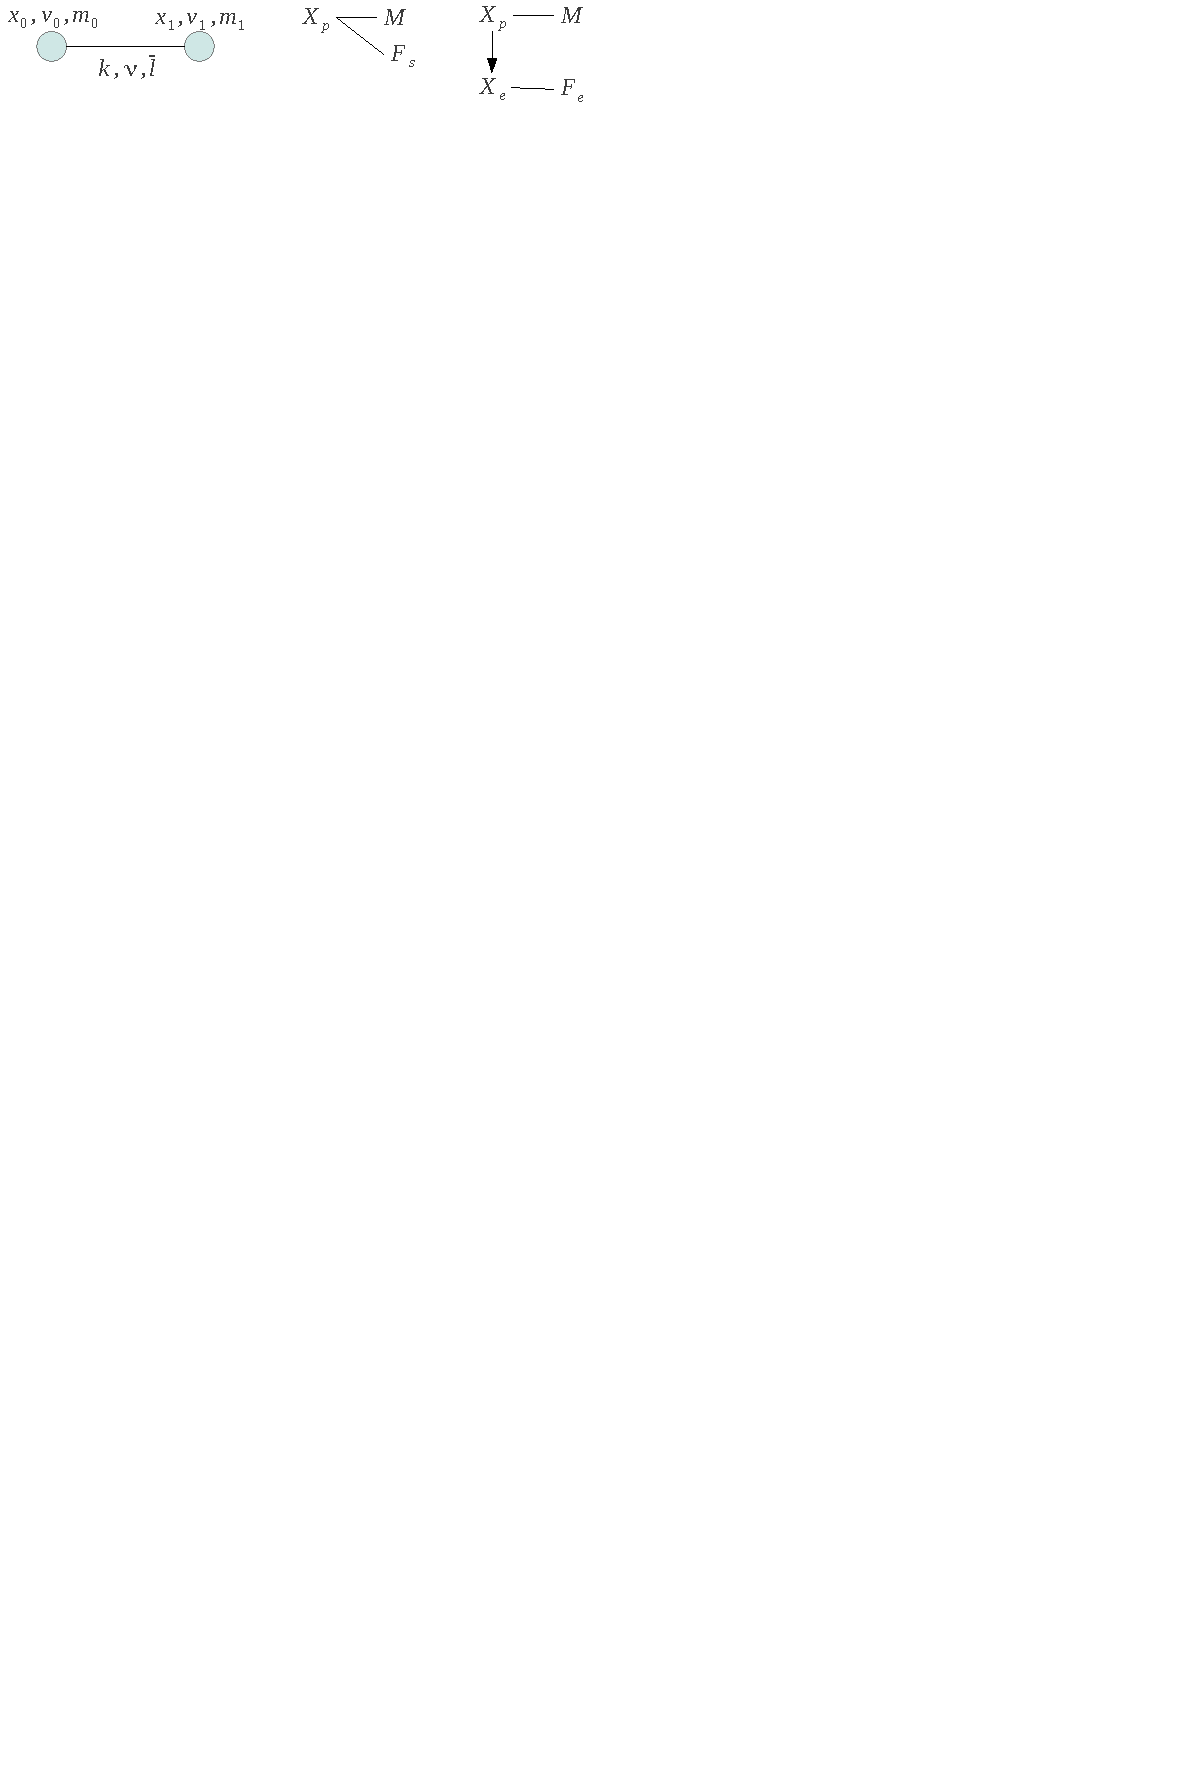
\includegraphics[clip,trim=0mm 285mm 155mm 0mm]{mass-spring.pdf}
   \caption{Two masses and a spring.} \label{fig mass-spring}
 \end{subfigure}
 \begin{subfigure}[t]{0.3\linewidth} \centering
   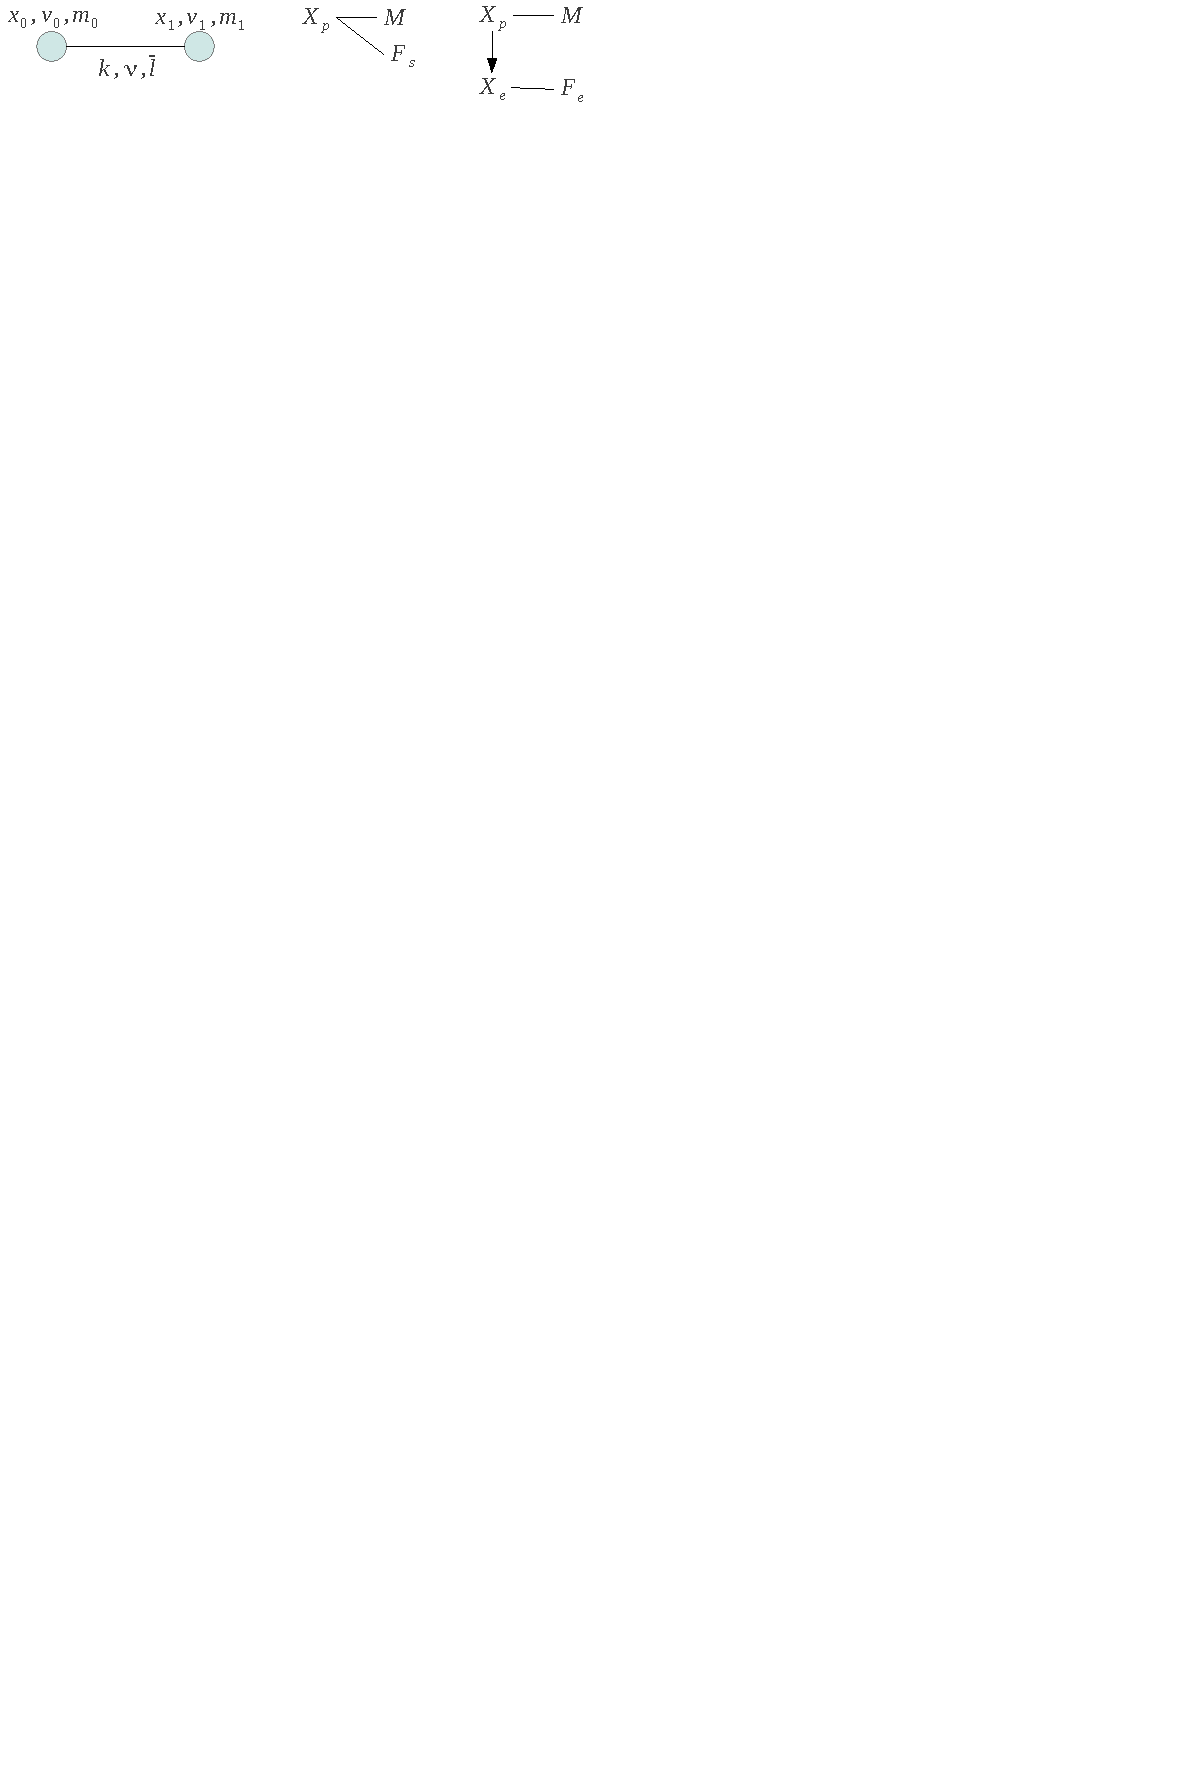
\includegraphics[clip,trim=50mm 285mm 130mm 0mm]{mass-spring.pdf}
   \caption{Traditional \sofa{} scene graph.} \label{fig mass-spring-traditional}
 \end{subfigure}
 \begin{subfigure}[t]{0.3\linewidth} \centering
   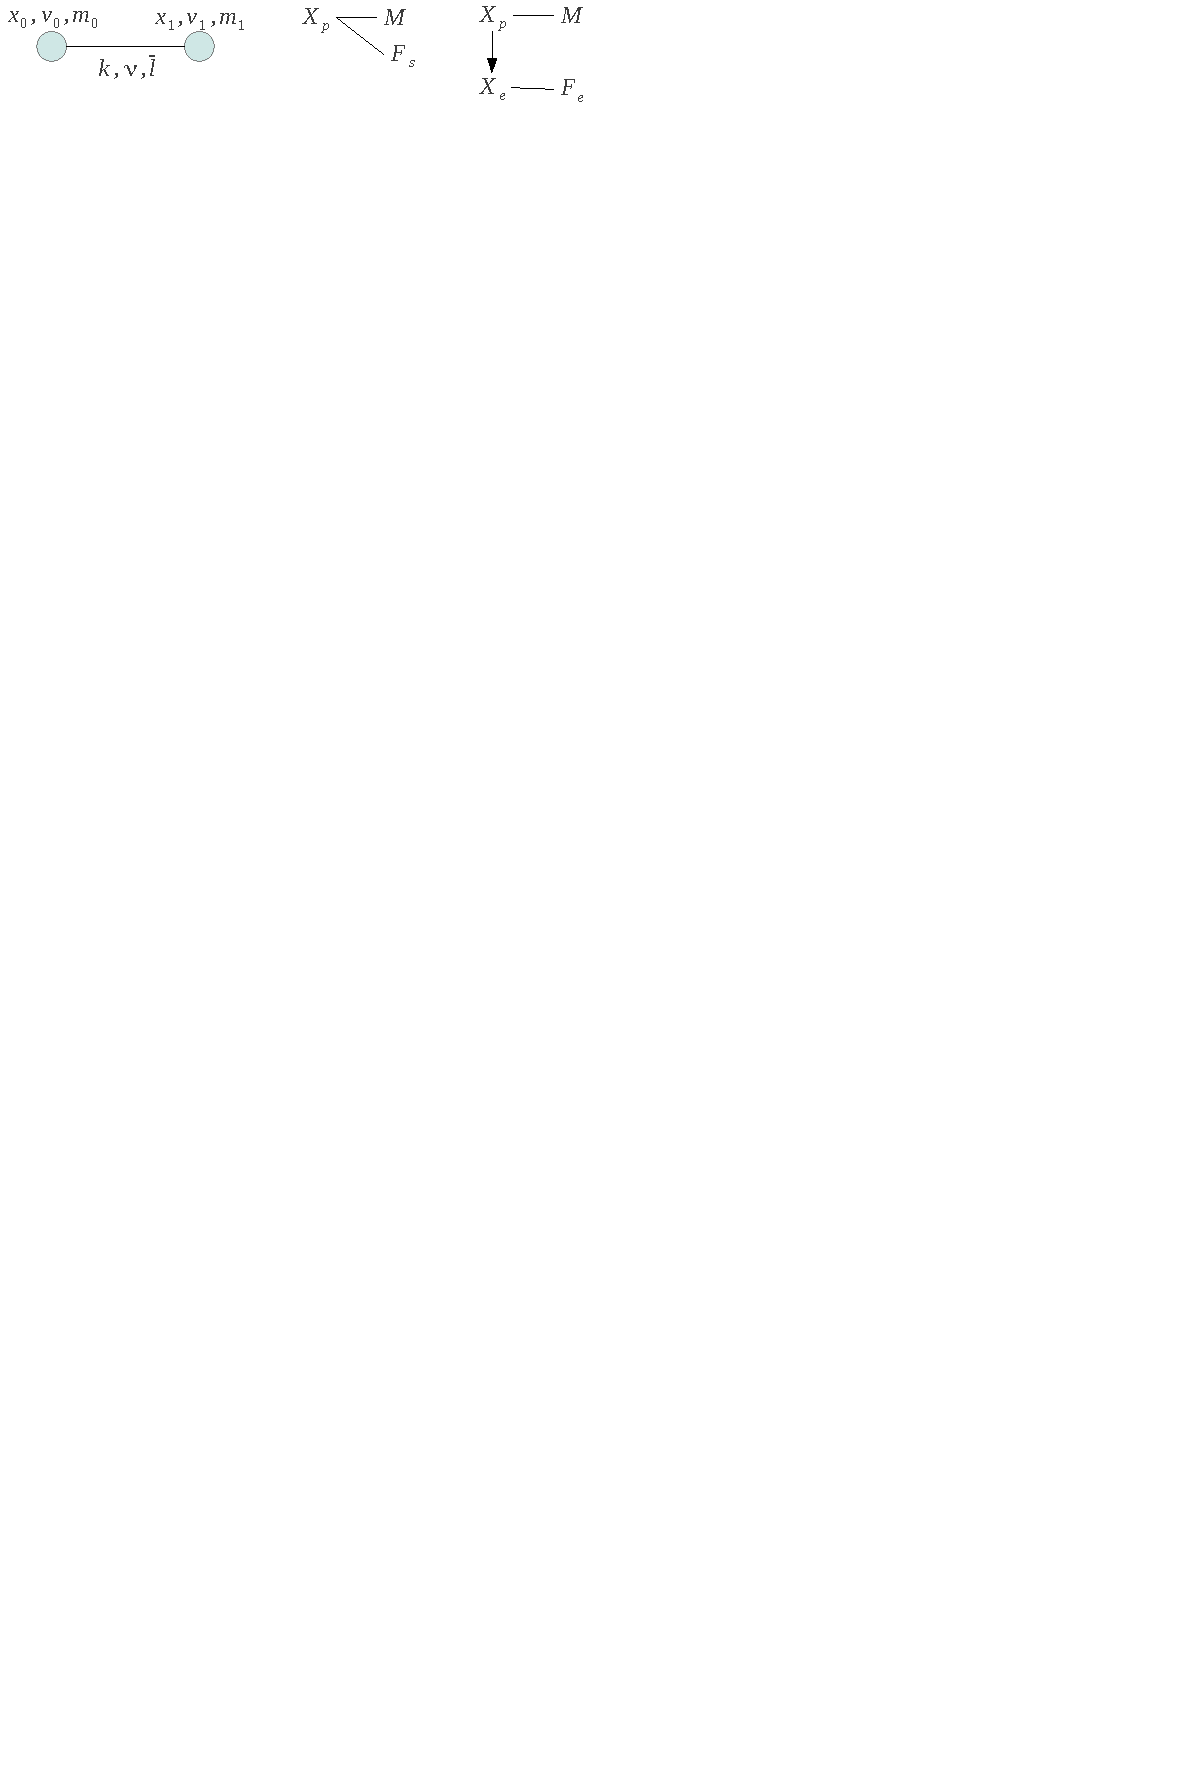
\includegraphics[clip,trim=80mm 280mm 100mm 0mm]{mass-spring.pdf}
   \caption{A more modular data structure.} \label{fig mass-spring-flexible}
 \end{subfigure}
 \caption{Improved modularity. $X$ denotes a state component, $M$ is mass, and $F$ a force field, while arrows represent mappings. $X_p$ represents particle positions while $X_e$ represents spring extensions, and $F_s$ represents spring forces while $F_e$ represent extension forces.}
 \label{fig modularity mass-spring}
\end{figure}



\section{Three-layer Continuum Mechanics}
The Flexible plugin provides components to model Lagrangian deformable solids using three layers, as illustrated in fig.\ref{fig tree levels}.
We present an overview of these and refer to subsequent sections for more detail.
\begin{figure}
 \centering
 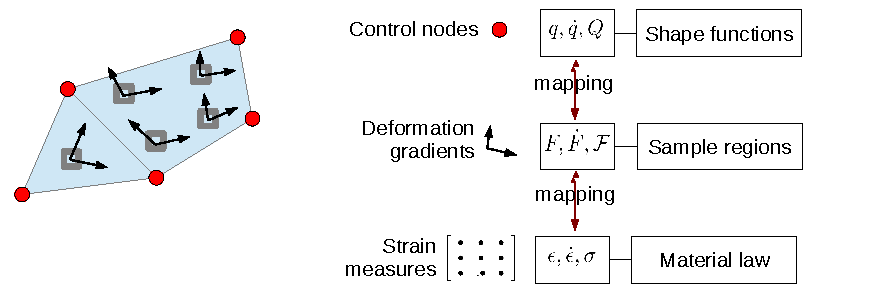
\includegraphics[height=0.3\linewidth]{threeLevels.pdf}
 \caption{The deformable solid in the left is modeled using the three kinematic levels shown in the right.
 The red disks, the grey squares and the local frames respectively represent the control nodes, the integration points and the deformation gradients at these points.
 }\label{fig tree levels}
\end{figure}

The top level contains the control nodes, which carry the independent degrees of freedom (DOF) of the object in state vectors $\vect \dof$ 
and $\dot{\vect\dof}$ for positions and velocities, respectively . 
In this example we use standard finite element (FE) nodes, but these could be any set of generalized coordinates such as moving frames, or deformation modes.
The shape functions represent how the material space of the object is mapped to the world space, based on the DOF. They are discussed in sec.\ref{sec shape functions}.

The second level contains deformation gradients, which represent the local state of the continuum, like small reference frames painted on the object.
Each of these is typically influenced by several control nodes in the upper level.
Their basis vectors are orthonormal in the undeformed configuration, while departure from unity corresponds to compression or extension, and departure from orthogonality corresponds to shear.

The deformation gradients are computed using a mapping based on the control nodes and their associated shape functions.
Different mappings are used depending on the type of control nodes (points, frame, etc.) and shape functions (linear or higher level interpolation, RBF, etc.). These mappings are presented in sec.\ref{sec deformation mapping}.
The deformation gradients are evaluated at carefully chosen sample points associated with object regions, which volumes are used to compute spatial integrals across the object. Sampling and quadrature are discussed in sec.\ref{sec quadrature}.

The lower level contains measures of deformation, typically called strains.
Each of these typically correspond to one deformation gradient at the upper level.
There are several ways of measuring deformation, including the well-known Cauchy strain, Green-Lagrange strain and corotational strain which for 3D objects are $3 \times 3$ symmetric tensors, or scalar values such as the determinant of the deformation gradient.
Different mappings are used to evaluate the different types of strain, as presented in sec.\ref{sec strain mapping}.

The constitutive law of the object material is applied at the lower level to compute stress $\stress$ based on strain $\strain$. 
More detail is given in sec.\ref{sec materials}.
The vector of stresses $\vect \stress$ is mapped upward to generalized forces $\vect \fdefograd$ homogeneous to deformation gradients, which are multiplied by the sample size and possibly other volume moments to integrate across the object volume.
These generalized forces are then mapped upward to node forces.


Mass can be integrated at the middle level using volume samples, or set at the top level.







%--------------------------------------------------------------------------------------------
\section{Shape functions} \label{sec shape functions}

\subsection{Shepard}

Shepard shape functions correspond to inverse distance weights (\url{http://en.wikipedia.org/wiki/Inverse_distance_weighting}).

They are defined as $\shapef_i(\mCoord)=1/|| \mCoord-\mCoord_i ||^p$ followed by normalization.

\subsection{Barycentric}

Barycentric shape functions are the barycentric coordinates of points inside cells (can be edges, triangles, quads, tetrahedra, hexahedra).
They achieve first order consistency: $\mCoord= \sum \shapef_i \mCoord_i$
 
\subsection{Natural Neighbors}

Natural neighbor interpolants are based on Voronoi diagrams.
Currently, Voronoi diagrams are computed from an image (a rasterized object).

\subsection{to do}

\begin{itemize}
 \item higher order FEM
 \item clarify material vs. spatial coordinates
 \item 
\end{itemize}







%--------------------------------------------------------------------------------------------
\section{Deformation mapping} \label{sec deformation mapping}

\subsection{linear mapping}

Child positions are computed as a linear combination of parent node dofs.
For instance, the mapping from points to points is : $\p = \sum_i w_i (\vdof - \vdofinit)$.
The mapping from affine frames to points in homogeneous coordinates is : $\p = \sum_i w_i \vdof \vdofinit^{-1} \pinit$.

\subsection{Extension mapping}

\subsection{Distance mapping}

\subsection{Log rigid mapping}

\subsection{Relative rigid mapping}

\subsection{Triangle deformation mapping}

\subsection{to do}

\begin{itemize}
 \item Moving Least squares
 \item non-linear skinning
 \item clarify material vs. spatial coordinates
 \item model plasticity/control using relative mappings
 \item 
\end{itemize}





%--------------------------------------------------------------------------------------------
\section{Strain mapping} \label{sec strain mapping}

\subsection{Green-Lagrangian strain}

The strain is mapped from the deformation gradient as : $\mat{E} = (\defograd^T\defograd - \mat{I} )/2$.
Here the strain is stored into vectors using Voigt notation. In 3d, we have: $\strain = [\strain_{xx} , \strain_{yy} , \strain_{zz} , 2\strain_{xy} , 2\strain_{yx} , 2\strain_{xz} ] $
The energy conjugate SPK stress vector is $\stress = [\stress_{xx} , \stress_{yy} , \stress_{zz} , \stress_{xy} , \stress_{yx} , \stress_{xz} ] $

\subsection{Corotational strain}

The rigid displacement $\mat{R}$ is first extracted from the deformation gradient using, for instance, SVD, polar or QR decomposition.
Then, supposing that the non-rigid deformation $\mat{R}^T \defograd$ is small enough, we can apply the Cauchy strain formulation:  $\mat{E} = [\mat{R}^T \defograd + \defograd^T \mat{R} ) /2 - \mat{I} $.


The geometric stiffness contribution does not seem necessary because it does not visually change the behaviour but can compromise the stability.
\begin{itemize}
\item analytical QR decomposition jacobians given in "Finite Random Matrix Theory, Jacobians of Matrix Transforms (without wedge products)", Alan Edelman, 2005, http://web.mit.edu/18.325/www/handouts/handout2.pdf (UNSTABLE)
\item Polar decomposition gradients inspired by Jernej Barbic, Yili Zhao, "Real-time Large-deformation Substructuring" SIGGRAPH 2011 (UNSTABLE)
\item SVD gradients given in Christopher Twigg, Zoran Kacic-Alesic, "Point Cloud Glue: Constraining simulations using the Procrustes transform", SCA'10 (QUITE STABLE)
\end{itemize}

\subsection{Principal stretches}

The principles streches $\mat{U}$ are directly extracted from the deformation gradient using a SVD, where the principal streches can be deduce from the eigen-values.
Note that the corresponding stress is also represented by 3 values, so isotropic materials are not applicable.

The geometric stiffness contribution is important.
\begin{itemize}
\item SVD gradients given in T. Papadopoulo, M.I.A. Lourakis, "Estimating the Jacobian of the Singular Value Decomposition: Theory and Applications", European Conference on Computer Vision, 2000 (STABLE)
\end{itemize}

\subsection{Diagonal strain}

The diagonal strain $\mat{D}$ is the principles streches + additional terms to allow anisotropic materials. 


\subsection{Invariants of deformation tensor}

The elastic energy of some materials are expressed using the three invariants of the right Cauchy deformation tensor $\mat{C}=\defograd^T \defograd$ :

\begin{itemize}
 \item $I1(\mat{C}) = trace(\mat{C})$
 \item $I2(\mat{C}) = ( trace(\mat{C}^2)+trace(\mat{C})^2 )/2$
 \item $I3(\mat{C}) = det(\mat{C})$
\end{itemize}

In practice, deviatoric invariants are used:
\begin{itemize}
 \item $\tilde{I1}(\mat{C}) = I1(\mat{C})/det(\defograd)^{2/3}$
 \item $\tilde{I2}(\mat{C}) = I2(\mat{C})/det(\defograd)^{4/3}$
\end{itemize}

Invariants are homogeneous with energies, so we use their squared roots as the state vectors.

\subsection{to do}

\begin{itemize}
 \item fix undefined invariants for inverted/flat elements
 \item 
 \item 
\end{itemize}







%--------------------------------------------------------------------------------------------
\section{Materials} \label{sec materials}

\subsection{Hooke Force field}

Hooke materials have linear strain/stress relationships: $\stress=\mat{H}\strain$. 
The potential energy is $W= \int_{\volume} \strain^T\mat{H}\strain /2$. 

\subsection{Mooney Rivlin}

The potential energy is $W= \int_{\volume} [ C1 ( I1 - 3)  + C2 ( I2 - 3) ]$, where $C1$ and $C2$ are material constants.

\subsection{Volume preservation}

Possible energy formulations for volume conservation are :
\begin{itemize}
 \item $W= \frac{k}{2} \int_{\volume} log( det(\defograd) )^2$
 \item $W= \frac{k}{2} \int_{\volume} (det(\defograd)-1)^2$
\end{itemize}
where $k$ is the bulk modulus.

\subsection{to do}

\begin{itemize}
 \item merge with implemented fem materials (Costa, Arruda-Boyce, NeoHookean, Veronda)
 \item 
 \item 
\end{itemize}

\newpage
%--------------------------------------------------------------------------------------------
\section{Quadrature} \label{sec quadrature}

Quadrature points are sampled using one of the GaussPointSampler component.
Currently, samplers can take meshes or images as inputs.

Quadrature methods estimate integrals using a sum of weighted evaluations at sample positions: $\int_{\volume} f(\pinit) d\volume \approx \sum_i v_i f(\pinit_i) $

\subsection{Mid-point}

The simplest method is to take one point per region and weight the value by its volume.
This is exact only for constant functions (e.g., elastic energy in a first order tetrahedral FEM)

\subsection{Gauss-Legendre}

Several points are used to approximate the intergral of higher order functions.
Currently only first order Gauss-Legendre quadrature on hexahedra is implemented.

\subsection{Elastons}

The idea is to decompose $f$ on a basis: $f(\pinit)=\mat{c}(\pinit_0) \polynomial{(\pinit-\pinit_0)}{*}$, 
where $\mat{c}$ are the coeficients and $\polynomial{()}{*}$ the basis vector (for instance the first order polynomial basis $[1,x,y,z]$).
The integral is then estimated as  $\int_{\volume} f(\pinit) d\volume \approx \mat{c}(\pinit_0)  \int_{\volume} \polynomial{(\pinit-\pinit_0)}{*} d\volume = \sum_i v_i c_i(\pinit_0) $
where the coeeficient $v_i$ part can be precomputed using an arbitrary fine discretization.

\subsection{to do}

\begin{itemize}
 \item Newton Cotes
 \item Finish implementation of elastons. Required instanciations for all force fields..
 \item 
\end{itemize}

\appendix

\section{Background - to rephrase}
This section contains material which needs rephrasing.

The numerical simulation of continuous deformable objects is based on a discrete number of independent degrees of freedom (DOFs) which we will call the nodes. They are kinematic primitives (can be points, frames, etc.).

Nodes are associated with shape functions which are combined to produce the displacement function of material points in the solid.

We introduce the following notations:
\begin{itemize}
 \item $\vdofinit$, $\vdof$ and $\fdof$ : the initial positions, current positions, and forces of the nodes.
 \item $\mCoord$ : the material coordinates of a point according the chosen parameterization of the solid.
 \item $\pinit(\mCoord)$, $\p (\mCoord)$ : the initial and current position of a point in space
 \item $\disp (\mCoord) =\p-\pinit$ : the displacement of a point
 \item $\shapef_i(\mCoord)$ : the shape function associated with node $i$
\end{itemize}

The local deformation is computed by differentiation with respect to material coordinates. The deformation gradient is: $\defograd = \partial \p / \partial \mCoord$.

The elastic deformation is described using a strain measure based on the deformation gradient. 

These three stages can be modeled using \sofa{} mappings:

\begin{equation}
\left. \begin{array}{ccccc}
\mbox{Nodes}  & \MappingArrows &   \mbox{Deformation gradients} & \MappingArrows &  \mbox{Strains}
\end{array}\right. 
\end{equation}

The elastic potential energy is computed from the strain. 

After spatial integration (quadrature), we obtain associated forces (total stress), that can be back propagated to the nodes using transposed jacobians.

\begin{equation}\label{eq:f}
 \vfdof = - \frac{\partial \W}{\partial \vdof}^T =  - \Jt_0\Jt_1 \int_{\volume} \stress
\end{equation}

Force variations are updated at each mapping by combining material and geometric stiffnesses. For a mapping from $p$ to $c$, we have:

\begin{equation}
 \delta(\vfdof_p) = ( \Jt \K_c \J + \frac{\partial \Jt}{\partial \vdof_p} \vfdof_c ) \delta(\vdof_p) 
\end{equation}

\newpage
%--------------------------------------------------------------------------------------------
\section{Scene graph}

\begin{itemize}
 \item \textbf{State =} nodes
 \item Shape function

 \item \textbf{ELASTICITY:}
  \begin{itemize}
  \item Gauss point sampler
  \item \textbf{State =} deformation gradients
  \item \textbf{Mapping =} deformation mapping

  \item \textbf{MATERIAL:}
    \begin{itemize}
    \item \textbf{State =} strains
    \item \textbf{Force field}
    \item \textbf{Mapping =} strain mapping
    \end{itemize}
  \end{itemize}

 \item \textbf{MASS:}
    \begin{itemize}
    \item \textbf{State =} points 
    \item Mass
    \item \textbf{Mapping =} deformation mapping
    \end{itemize}
 \item \textbf{COLLISION:}
    \begin{itemize}
    \item \textbf{State =} points 
    \item \textbf{Mapping =} deformation mapping
    \end{itemize}
 \item \textbf{VISU:}
    \begin{itemize}
    \item \textbf{State =} points 
    \item \textbf{Mapping =} deformation mapping
    \end{itemize}

\end{itemize}





\section{Requirements}

SOFA Packages:
The following must be enabled in sofa-local.prf
\begin{itemize}
\item (depends on nothing)
\end{itemize}

SOFA Plugins:
The following must be loaded in your SOFA instance
\begin{itemize}
\item Flexible
\end{itemize}

\section{Scene Settings}

\subsection{Required Settings}

\begin{componentoption}{RequiredExampleSetting}
A description of what this setting controls, and any special information the user should know about it. Required settings are those that need to be specified by the user in order for the component to function. If your component doesn't have any required settings, leave this section blank. The below "value type" is the type that is expected by the component. "Aliases" are other strings that can be specified in the scene file for this setting. These are defined in the code using "addAlias()".
\valuetype{string}
\aliases{requiredexamplesetting}
\end{componentoption}


\subsection{Optional Settings}

\begin{componentoption}{OptionalExampleSetting}
A description of what this setting controls, and any special information the user should know about it. Optional settings can be specified by the user in order to change the default behaviour of the component. The below "Default Value" is the value given to the setting if the user doesn't specify anything.
\valuetype{bool}
\defaultvalue{false}
\aliases{optionalexample, optionalsetting}
\end{componentoption}

\section{Scene Data}

\subsection{Required Data}

\begin{componentoption}{RequiredExampleData}
Data is usually a link to something in another component. Required data must be specified in order for the component to function.
\valuetype{ExampleType}
\end{componentoption}

\subsection{Optional Data}

\begin{componentoption}{OptionalExampleData}
Data is usually a link to something in another component.
\valuetype{ExampleType}
\aliases{OptData}
\end{componentoption}

\subsection{Output data}
Output data is generally not defined in the component, but is linked to by other components.

\subsection{Example File}
path/to/an/example/file.scn

\end{document}
